\section{Question 4}

\subsection{Task}
Simulate the Langton’s ant. Look up Wikipedia about what this problem is. Make sure you provide the formulation, program implementation and sample images to verify the behavior of the ant motion in the box. Consider a box of size $64*64$ for


\subsection{Solution}

Link to the GitHub repository for this question: \href{https://github.com/Xerefic/MM2090-Solutions/tree/master/Final_Assignment/question_4}{GitHub} \footnote{Repo: \url{https://github.com/Xerefic/MM2090-Solutions/tree/master/Final_Assignment/question_4}}

\subsubsection{Rules}\footnote{Source: \url{https://en.wikipedia.org/wiki/Langton\%27s_ant}}
Initialize the state space of dimensions $64*64$ with all 0s, i.e., black pixels. Arbitrarily identify the starting location of the and update according to:
\begin{itemize}
	\item At a white square, turn 90° clockwise, flip the colour of the square, move forward one unit,
	\item At a black square, turn 90° counter-clockwise, flip the colour of the square, move forward one unit.
\end{itemize}

\subsubsection{Approach}
At every time step, to keep track of the orientation of the ant, I exploited the use of residues of 4. So basically, computed the modulo of \textbf{orient} and 4 after every update. Following which the location of the ant at the start of the $\left(t+1\right)^{th}$ time-step is calculated. Accordingly, the pixels are updated. The states are sampled every so often to observe the actions of the ant.


\subsubsection{Requirements}
Language of choice: python
\begin{lstlisting}[language=bash]
	pip3 install numpy
	pip3 install matplotlib
	pip3 install opencv-python
\end{lstlisting}

\subsubsection{Observation}
After running the simulation several times, one can observe that the state evolves exactly in a similar manner every time. During the first few moves, the ant moves predictably in a symmetric manner. As the time progresses, the state appears chaotic resembling an unsymmetric disc. At around 10000 time-steps, the ant reaches an order of repetition, a sequence of 104 steps which the ant repeats to infinity. \\
Every simulation resembled the exact same start state followed by the repeating highway. Although there is no conclusive proof that this occurs for every start state, the trajectory is unbounded in every case.

\subsubsection{Output}
Please find attached the video of the states.

\begin{table}[!ht]
	\begin{center}
		\begin{tabular}{ | c | c | }
			\hline
			STATE & TIMESTEPS \\ \hline
			
\includegraphics[width=25mm, height=25mm]{question_4/Iteration-0.eps} & 
				0 \\ \hline
			
\includegraphics[width=25mm, height=25mm]{question_4/Iteration-100.eps} &
				100 \\ \hline
			
\includegraphics[width=25mm, height=25mm]{question_4/Iteration-200.eps} &
				200 \\ \hline
			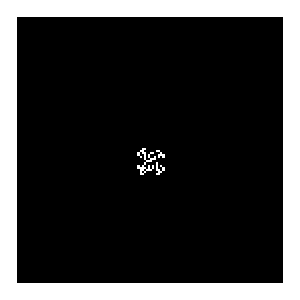
\includegraphics[width=25mm, height=25mm]{question_4/Iteration-500.eps} &
				500 \\ \hline
			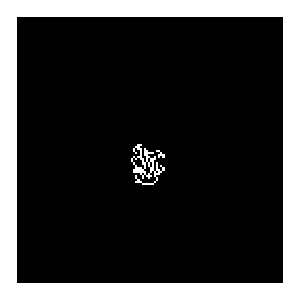
\includegraphics[width=25mm, height=25mm]{question_4/Iteration-1000.eps} &
				1000 \\ \hline
			
\includegraphics[width=25mm, height=25mm]{question_4/Iteration-5000.eps} &
				5000 \\ \hline
			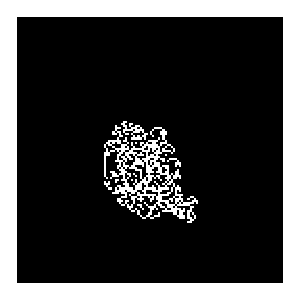
\includegraphics[width=25mm, height=25mm]{question_4/Iteration-10000.eps} &
				10000 \\ \hline
			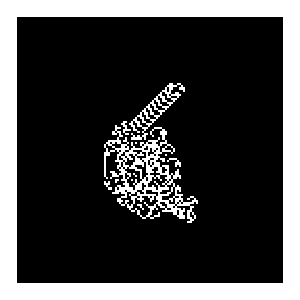
\includegraphics[width=25mm, height=25mm]{question_4/Iteration-11000.eps} &
				11000 \\ \hline
			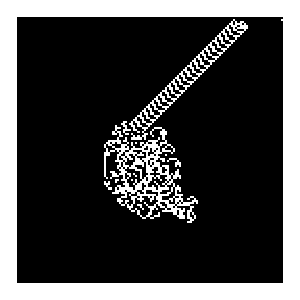
\includegraphics[width=25mm, height=25mm]{question_4/Iteration-19000.eps} &
				19000 \\ \hline
		\end{tabular}
	\end{center}
\caption{Simulation of States}
\end{table}

\clearpage
\subsection{Code}
\lstinputlisting{question_4/question4.py}

